
%The goal of this Chapter is to show how \name can improve the traditional top-down analysis method. Usually, researchers start from a deep comprehension of the theoretical problem and draw a model of the system. This model is exploited to formulate hypothesis and even if further knowledge about the implementation experience may support this method, this approach is traditionally top-down. Section \ref{sec:empirical-research} shows there is a lack in Computer Science about system evaluation. However, when the subject of the research are complex system, it is hard to formulate and prove hypothesis that are only based on he knowledge of the model and empirical evaluation becomes useful.

In this Chapter we present an evaluation of \name Baselines (See Chapter \ref{sec:baselines}) in order to demonstrate how \name can extend the traditional hypothesis-based research, towards the Systematic Comparative Research approach we introduced in Chapter \ref{chap:problem-settings}. In section \ref{sec:experimental-setting} we present our assumptions and we describe the Experimental Setting. In Section \ref{sec:experiment-design} we introduce the method to properly design experiment and two experiment set executed on \name Baselines: SOAK Tests in Subsection \ref{sec:soak-es} and Step Response Stress test in Subsection \ref{sec:step-es}. Finally, we present the experiment results respectively for SOAK test in Section \ref{sec:soakres} and for the Step Response Test in Section \ref{sec:stressres}.

The aim of SOAK tests is showing the problem dimension of traditional top-down analysis over complex software system like RSP Engine, even for simple hypothesis, and consequently demonstrate that we need \namens. Instead, the Step-Response tests are designed to show \name potential, and provide a simple case of analysis inspired by the Systematic Comparative Research Approach.

\section{Experiment Design}\label{sec:experiment-design}

Experiment design (ED) means project our experiment in order to prove or refute one or more hypothesis, evidencing the behaviour of the system in the context that those hypothesis involves. ED starts with some assumptions, which compose the  Experimental Setting. Researchers formulate hypothesis on the base of these assumptions, Figure \ref{fig:experiment-design} summarises the collocation of ED within the Top-down approach.

\begin{figure}[tbh]
  \centering
	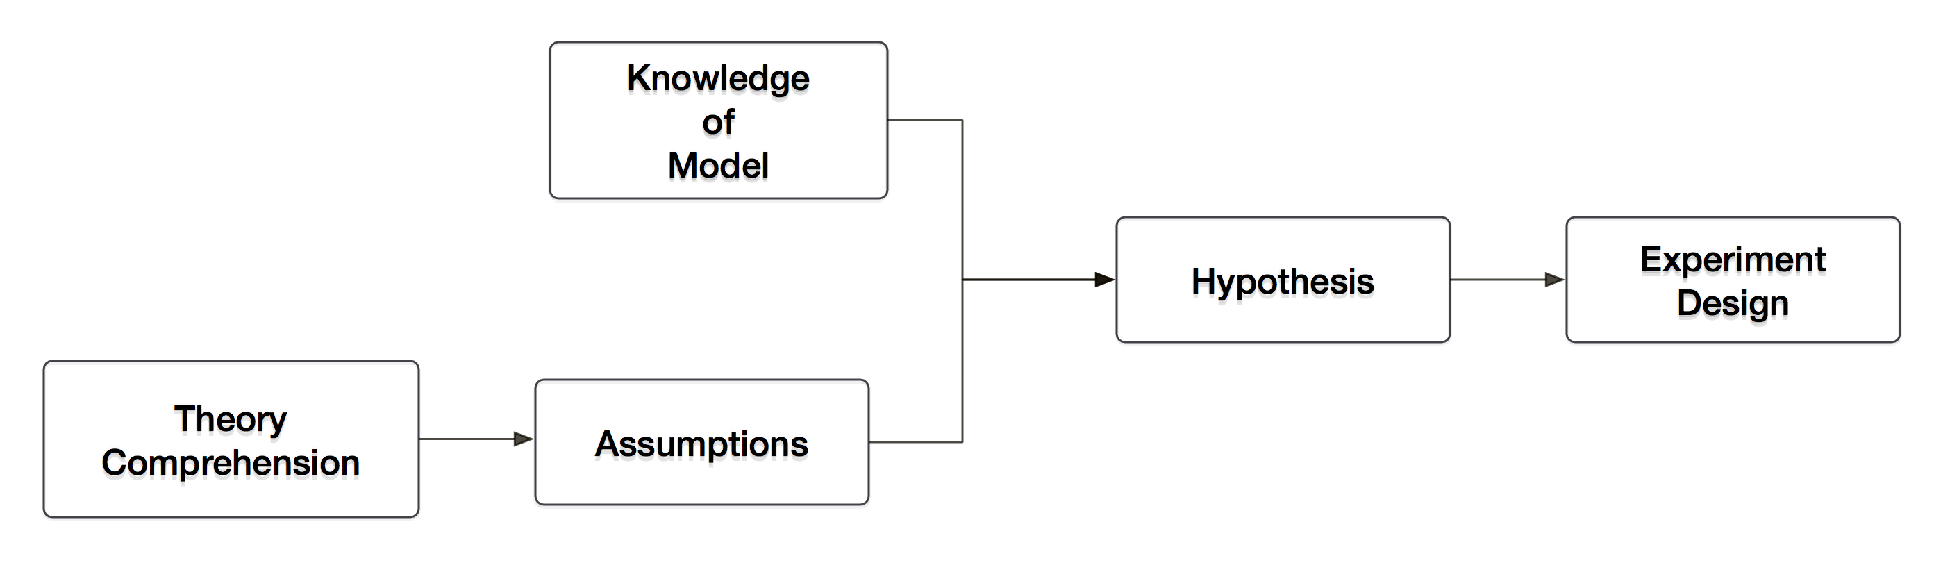
\includegraphics[width=\linewidth]{images/experiment-design}
	\caption{Traditional Experiment design workflow} 
  	\label{fig:experiment-design}
\end{figure}


From a theoretical point of view we decide to study RSP Engine facing their nature of linear dynamic system.(see Section \ref{sec:sfp}). Experiment design requires to point out which variable are observed. We simplify the study analysing their behaviour in term of Latency and Memory, which is the minimal meaningful measurement set for an RSP Engine (Chapter \ref{chap:heaven}).

In Chapter \ref{chap:heaven} we describe the experiment tuple: $<\mathcal{D}, \mathcal{T},\mathcal{E}, \mathcal{Q}>$ , where briefly:
\begin{itemize}
\item $\mathcal{E}$ is the RSP Engine
\item $\mathcal{D}$ is the Dataset 
\item $\mathcal{T}$ is the Ontology
\item $\mathcal{Q}$ is the Query that $\mathcal{E}$ continuously answers.
\end{itemize}

In this Section we present our choices about the four elements that compose an experiment, upon which the evaluation is built

\subsection{Engine $\mathcal{E}$}

%. Top-Down investigations are commonly hard, and they become even harder for commercial solutions.
The architecture complexity of mature RSP Engines like the C-SPARQL Engine or CQELS is high, and can not be easily faced in order formulate hypothesis of comparison. However, the purpose of this evaluation is showing how \name can improve the research over RSP Engine. Thus, we can simplify the research survey evaluating less complex systems. To this extent we design and implement the Baselines (Section \ref{sec:baselines}) and we evaluate them as the RSP Engines $\mathcal{E}$ subject of our experiments. 

In Chapter \ref{chap:problem-settings} we describe which requirements guarantee that an RSP Engine is a baselines: Simplicity, Elementarily, Relevance and Eligibility (SERE properties) legitimate the evaluation. Thus, they can be considered as a simple term of comparison for further research on Stream Reasoning systems and this investigation can be followed as guideline.
 
The four baselines differ for two characteristics: RDF Stream Model and Reasoning architecture. The Table \ref{tab:baselines-names} summarises these few but well determined differences, naming the four baselines for the evaluation:\begin{table}[htb]
\scriptsize
\centering
\begin{tabular}{c|cc} % creating eight columns
	\hline
         & Naive & Incremental\\
	\hline
	Graph        &  B1      & B2\\
	Statment   &  B3   & B4\\
	\hline % inserts single-
\end{tabular}
\caption{Naming convention of the four baselines, further details in Section \ref{sec:baselines}}
\label{tab:baselines-names}
\end{table}

\noindent Among these four configurations we can formulate simple hypothesis, stating which approach is better then an other one within an experiment. Notice that we have a complete model of the baseline systems and we also know many implementation details that can help during the analysis . We can exploit the know-how about their internal mechanisms, described in Section \ref{sec:baselines-impl}, to lead our analysis from hypothesis formulation towards empirical results. 

\subsection{Dataset $\mathcal{D}$ and Ontology $\mathcal{T}$}\label{sec:dataset}

\noindent The Dataset  $\mathcal{D}$ and the Ontology $\mathcal{T}$ must be chose to ensure baselines Simplicity, as stated in Section \ref{sec:baselines}. 

The RDF Streams (details in Section \ref{sec:rdfstream}) $\mathcal{D}$ used in the experiments are obtained streaming in different ways the data generated with LUBM  \cite{Guo2005}. Consequently we chose LUBM ontology\footnote{http://swat.cse.lehigh.edu/onto/univ-bench.owl} as $\mathcal{T}$ for all the experiment. We assume that the ontology does not change over time, therefore the materialisation of $\mathcal{T}$ is computed before starting the experiment and the RSP engine does not have to perform this task. 

It is worth to discuss the choice of using data from LUBM (Section \ref{sec:lubm}) over SRbench (Section \ref{sec:srbench}) and LSbench (Section \ref{sec:lsbench}). The first one has data, which are not adequate for the experiments, since they do not require any reasoning. The SRbench data, on the contrary, requires reasoning, but, being real-data, do not have the possibility to be scaled up and down. Moreover, this choice is in line with previous works on Stream Reasoning \cite{DBLP:conf/semweb/UrbaniMJHB13}. 

Being LUBM static data, we exploit the \textit{RDF2RDFStream} component of the \textsc{Test Stand} that takes care to adapt the data generate by LUBM to a streaming scenario (see Section \ref{sec:streamer-impl}). \textit{RDF2RDFStream} is responsible to build $\mathcal{D}$ w.r.t. $\mathcal{T}$. As detailed in the relative section it is able to scale both in terms of dimension of the dataset and the reasoning effort. The component can be set up to obtain an RDFStream where the number of triples with the same timestamps follows a given discrete function. %Section \ref{sec:streamer-impl} contains all the details about the implementation and the usage of this particular \textsc{Streamer}. %e' veramente il timestamp quello?

\subsection{Query $\mathcal{Q}$}\label{sec:query}
 
The the query $\mathcal{Q}$ used in our experiment depends on the reasoning approach of the RSP Engine in use. Actually, all  experiments uses variants of the basic identity query that continuously asks for the materialisation of the current sliding window $\omega$, which differ from the sliding factor $\beta$.\\

\begin{center}
\raggedright
REGISTER QUERY Q AS \\
SELECT ?s ?p ?o \\
FROM STREAM S [RANGE $\omega$ STEP $\beta$]\\
WHERE {?s ?p ?o}\\
UNDER $\rho$DF ENTAILMENT REGIME
\label{code:query}

\end{center}
Query: \ref{code:query}: Query $\mathcal{Q}$ registered to the \name Baselines.\\


The Baseline B1 and B3 exploit the Naive Reasoning approach and thus the query \ref{code:query} is implemented in order to output the snapshot of the entire window at each slide of the window. On the other hand, the Baselines B2 and B4 exploit the Incremental Reasoning approach and thus implement the query \ref{code:query} in order to output the ir-streams at each window slide.

The entailment regime of the RSP Engines influence performances. For this reason we take $\rho$DF  \cite{DBLP:conf/esws/MunozPG07} as their entailment regime, because several works in the field \cite{DBLP:conf/semweb/UrbaniMJHB13} choose this as the minimal meaningful task for a Stream Reasoner. In particular, $\rho$DF is the RDF-S fragment that reduce complexity while preserving the normative semantics and core functionalities.

%We describe in details the content of the SOAK (Section \ref{sec:soak-es}) and the Step Response tests (Section \ref{sec:step-es}), providing a lecture key for the experiment results.

\section{Experiment Set-Up}

The \textit{RDF2RDFStream} allows to control the triple distribution in the RDFStream, thus it is possible to build experiment with different input RDF Stream. We design set of SOAK Tests to evaluate the Baselines, which can evidence how as baseline behaves over very long executions providing an image of the RSP Engine dynamics. Moreover, in order to show \name potential, we design a small set of Stress Test, which belongs to the Step Response subcategory. In summary:

\begin{itemize}
\item \textbf{SOAK}: the number of contemporary triple in the RDFStream does not change during the experiment.
\item \textbf{Step Response} the number of contemporary triple suddenly changes during the experiment, usually increasing of a degree of magnitude.
\end{itemize}

We execute the experiment on each \name Baseline, so we design experiment basing which query is registered to them. Experiment queries differ for the size $\omega$ of the sliding window. In particular, we use windows in which $\omega$ is an integer multiple of the slide parameter $\beta$ of the window, i.e., it holds that $\omega = \beta * N$. In other words, $N$ is the number of \textsc{CTEvents} that the window contain. 

Moreover, Section \ref{sec:baselines-impl} shows how the proposed baselines take advantage of the ability of Esper to be temporally controlled by an external agent\footnote{\url{http://esper.sourceforge.net/esper-0.7.5/doc/reference/en/html_single/index.html#api-controlling-time}} by sending time-keeping events to synchronise the internal time flow. All the triples in the \textit{CTEvent} are consider contemporary by the baselines and each \textit{CTEvent} can be seen as a proxy for the timing event. Together with the \textit{RDF2RDFStream} is possible to estimate the content of the current window in terms of number of RDF Triples in any moment of the experiment.

All experiment are execute 10 times oto reduce the presence of the outlier.

Further details about the two test sets in the following Sections \ref{sec:soak-es} for SOAK Test and \ref{sec:step-es} for Step Response tests.

\subsection{SOAK: Tests and Hypothesis}\label{sec:soak-es}

Soak testing show the system dynamics, injecting to the subject a constant and continuous input flow (see Section \ref{sec:software-testing}.  We control the number of contemporary triples in the RDF Stream trough the \textit{RDF2RDFStream} module. %Moreover, Section \ref{sec:query} describe how we variates the query between experiments.

SOAK Experiment are 30000 CTEvent long, each one of a fixed size, which depend on the specific experiment. Unlikely, it is not possible to foretell how many events are required in to reach the Steady State condition for each variable involved, especially memory. The Experiment Results show this in detail in Section \ref{sec:soakres}. Multiple attempts and empirical evaluation are the only way to set up the correct longness.

\begin{table}[htb]
\centering
\normalsize
 \begin{tabular}{l| ccccc}
	  	\hline
		\textsc{CTEvent}  &\multicolumn{5}{c}{Number of Slot}  \\
		Size  & 1 & 10 & 100 & 1000&10000 \\
		\hline	
		1 & 1& 10 & 100 & 1000&10000 \\
		10  & 10 & 100 & 1000&10000 \\
		100 & 100&1000&10000  \\
		1000 &1000 & 10000 \\
		10000&10000  \\
		\hline 
	\end{tabular}
	
	 \vspace{10pt}
	\caption{The number of triples in the window during the fifteen SOAK tests as a function of the Window size (in terms of $N$) and of the triples in each \textsc{CTEvent}.}
	\label{tab:soaktests}
\end{table}

\begin{table}[htb]
	\centering
	\normalsize
	\begin{tabular}{l | ccccc} % creating eight columns
	  	\hline
		Triple in & \multicolumn{5}{c}{Number of Slots}  \\
		Window  & 1 & 10 & 100 & 1000&10000\\
		\hline
		1  	 & 1\\
		10   & 10  & 1 \\
		100  & 100 & 10 & 1\\
		1000 & 1000& 100& 10& 1\\
		10000& 10000 & 1000& 100& 10& 1\\
		\hline % inserts single-line
	 \end{tabular}
	\caption{The number of triples in a \textsc{CTEvent} during the fifteen SOAK tests as a function of the Window size (in terms of $N$) and of the total triples in the active window, assuming one and only one \textsc{CTEvent} per slot.}
	\label{tab:soaktests-alt}
\end{table}

Table \ref{tab:soaktests} presents the fifteen SOAK tests we run for each baseline presented in Table \ref{tab:baselines-names}. The columns of the table are the different window sizes measured in terms of the values assumed by $N$ (see Section \ref{sec:query}).  Being $\beta=$ 100 ms., they correspond to a window that spans 100 ms., 1 sec., 10 sec. and 100 sec.. The rows are the different number of triples in each \textit{CTEvent} sent by the \textsc{RDF2RDFStream} to $\mathcal{E}$.% Notably, for all of them, we checked that $\mathcal{E}$ is responsive for the whole duration of the experiment. 

Table \ref{tab:soaktests-alt} is an alternative layout. The columns of the table are still contain the different window sizes measured in terms of the values assumed by the number of slots $N$, while the rows are the different number of triples in the active window. \\

Following the traditional research method, we formulate two naive hypothesis based on the knowledge we have of the model. The hypothesis to verify with SOAK experiments are:
\begin{itemize}
\item \textbf{HP.1} The Incremental reasoning approach is always better then the naive one.
\item \textbf{HP.2} The Graph-based model for RDFStream is always better then the Triple-based one.
\end{itemize}

Notice that the goal of our research is to show how \name helps RSP Engine analysis trough empirical evaluations. Hypothesis verification and top-down analysis are the subject of our survey, while our research question is:  "\textit{Can an engine test stands, together with queries, datasets and methods, support Systematic Comparative Research Approach for Stream Reasoning?}" %"Needs the Stream Reasoning research field a Test Stand like \name to investigate RSP Engines and sustain the research of such system with an Systematic Comparative Approach?"

\subsection{Step Response Tests}\label{sec:step-es}

Step Response testing allow to see how the system reacts to a sudden changing in the input condition (see Section \ref{sec:software-testing}). They are related to SOAK test, because they allow to study deeply the initial warm-up phase of the system. This set of experiments evidence the different responses of an RSP Engine if we move form an input condition to another instead of starting from scratch.

We design the step experiments concatenating two with total length of 400000 events, which means hours of execution for the system. For this reason we investigate only few configuration, all with 10  window slot size for all the four baselines. Table \ref{tab:steptests} summarises the step experiment set-up, where the step is positioned at the half of the execution, 20000 events.
\begin{table}[htb]
\centering
 \begin{tabular}{c|c|c}
	  	\hline
	  	&\multicolumn{2}{c}{CTEvent size}  \\
		Window Size & Initial Size & Final Size\\
		\hline
		\hline
		 10 & 10 & 100\\
		  10 & 100 & 1000\\
		 10 & 10 & 1000\\
		% 10 & 10 & 10000\\
		
		% 10 & 100 & 10000\\
		% 10 & 1000 & 10000\\
		\hline 
 \end{tabular}
 \caption{}
\label{tab:steptests}
\end{table}

We do not formulate hypothesis for Step experiments. The purpose of this test set is to show \name capabilities and not to offers a deep understating of the baselines. However, we comment the results evidencing the finding in the sections below.

\subsection{Execution Environment}\label{sec:execution-environment}

Before presenting experiment result a brief description of the execution environment is required. All experiment are executed exploiting a dedicated machine, an iMac mid-2011 with 12GB RAM and 3.6 Ghz of a Intel i5 64 Bit, which run OS X 10.10.2 Yosemite,. Since \name is developed with Java 7\footnote{http://www.oracle.com/technetwork/java/javase/javase7locales-334809.html}, we use the versione 1.7.0.71 of the JVM.
The execution happens in a controlled environment, which tries to reduce the number of disturbing elements like network, graphical interface and other running processes.

\section{SOAK Test Evaluation Results}\label{sec:soakres}

In this Section we present the Experiment results of the SOAK Test, trough the different levels of analysis introduced in Chapter \ref{chap:heaven} and detailed in Chapter \ref{chap:implementation-experience}. We face the hypothesis formulated in Section \ref{sec:soak-es} and provides many findings exploiting the analysis tools which support each level.

Notice that the Experiments with the CT Event Size  10000 a Single Slot do not terminate correctly due to an execution error. The reader please ignore the results of this experiment, which are not actually part of our evaluation.

\subsection{Level 0 - Dashboards}

\begin{figure}[tbh]
	\centering
	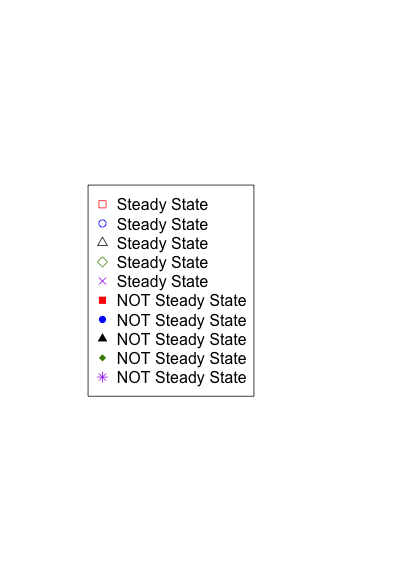
\includegraphics[width=\linewidth]{images/dashboard-legend}	
	\caption{Dashboard Legend} 
	\label{fig:dashboard-legend}
\end{figure}

The SOAK test results analysis starts with the high level dashboard view. Each dashboard presented is composed by two chart which shows in different form the relation between the different four baselines. Dashboard legend is fixed for all the following charts and reported in Figure \ref{fig:dashboard-legend}.

\begin{figure}[tbh]
	\centering
	%\includegraphics[width=\linewidth]{images/result_dashboard_ka}	
	\caption{Dashboard K=1 Split} 
	\label{fig:result_dashboard_ka}
\end{figure}

\begin{figure}[tbh]
	\centering
	%\includegraphics[width=\linewidth]{images/result_dashboard_kb}	
	\caption{Dashboard K=1 Multiplot} 
	\label{fig:result_dashboard_kb}
\end{figure}

\textbf{Dashboard One - Fixed Size \textsc{CTEvent} = 1} - How baselines behaviour changes if we fix the size of the \textsc{CTEvent} while we analyse the variation of the number of slot in the active window? Figures \ref{fig:result_dashboard_ka} and \ref{fig:result_dashboard_kb} shows this situation within a dashboard view. 

To better understand this analysis we refer to the experiment layouts of Table \ref{tab:soaktests-alt}. Fixing the \textsc{CTEvent} size while the Number of slot is changing means moving on the table diagonals, if \textsc{CTEvent} size = 1 indicates the latest one.
Observing Figure \ref{fig:result_dashboard_ka} we can appreciate that while the number of slots grows and thus the window size (in terms of triple) increases, all the baselines have a worsening in terms of Latency. Observing Figure \ref{fig:result_dashboard_kb} we can also individuate the worsening for the memory consumption, which is growing too. A first obvious insight may be that \textit{Bigger problem requires in general more resources}. Notice that the green point (Bx), it is not part of the chart for very small problems (1 Triple tumbling window).

\begin{figure}[tbh]
	\centering
	%\includegraphics[width=\linewidth]{images/result_dashboard_ewa}	
	\caption{Dashboard EW=10 Split} 
	\label{fig:result_dashboard_ewa}
\end{figure}

\begin{figure}[tbh]
	\centering
	%\includegraphics[width=\linewidth]{images/result_dashboard_ewb}	
	
	\caption{Dashboard EW=10 Multiplot}
	\label{fig:result_dashboard_ewb}
\end{figure}

\textbf{Dashboard Three - Fixed Number of Slot = 10} - How baselines behaviour changes if we fix number of slot in the active window while the size of the \textsc{CTEvent} changes? Figures \ref{fig:result_dashboard_ewa} and \ref{fig:result_dashboard_ewb} show this situation. This analysis means, w.r.t Table \ref{tab:soaktests-alt} layout, moving form the top to the bottom of the second column.

Observing the two Figures emerge two finding: (1) Latency worsening is still clearly visible in Figure \ref{fig:result_dashboard_ewa}, while the Memory ones requires Figure \ref{fig:result_dashboard_ewb} (2) The behaviour of the baselines becomes indistinguishable when the window size in terms of triple is grown too much. 

\begin{figure}[tbh]
	\centering
	%\includegraphics[width=\linewidth]{images/result_dashboard_proba}	
	\caption{Dashboard $EW*K=10000$ Split} 
	\label{fig:result_dashboard_proba}
\end{figure}

\begin{figure}[tbh]
	\centering
	%\includegraphics[width=\linewidth]{images/result_dashboard_probb}	
	\caption{Dashboard $EW*K=10000$ Multiplot}
	\label{fig:result_dashboard_probb}
\end{figure}

\textbf{Dashboard Two - Fixed Windows Size (Triples) = 10000 } - How baselines behaviour changes if we fix number triples within the active window? The analysis is summarized in the Figures \ref{fig:result_dashboard_proba} and \ref{fig:result_dashboard_probb}. Fixing the window size in terms of triple to 10000 means moving form the left to the right on the lowest row of Table \ref{tab:soaktests-alt}. Formally, it consist into maintain the product CTEvent size (K) and Slot Number (EW) constant to 10000 triples. Both the Figures report how the baselines performances seems depends only on the dimension of the active windows, indeed they are almost the same for all the compared experiments.

What Level 0 allows to state is there is no strong dominance of a Baseline w.r.t. the other ones in the provided analysis. Moreover, a week dominance can be observed in different steps both in term for Latency  and memory. The most clear example is in Figures \ref{fig:result_dashboard_ka} and \ref{fig:result_dashboard_kb} and in Figures \ref{fig:result_dashboard_ewa} and \ref{fig:result_dashboard_ewb} for medium size problems with Baseline B4. 
However the dominance is not absolute and changing experiment configuration may changes the result hierarchy. This observation refutes explicitly HP.2 formulated in Section \ref{sec:soak-es}, while HP.1 was not completely confirmed. There are experiments where the naive  reasoning  approach seems performing better than the incremental one, at least in term of Latency. 

The research over RSP Engines requires further analysis at deeper levels to  motivate these unexpected findings and \name makes this possible.

\subsection{Level 1 -  Statistical Values Comparison}

\begin{table}[htbp]
	\centering
	\scriptsize
	\subtable[Incremental]{%
		\begin{tabular}{l | ccccc} % creating eight columns
	  	\hline
		Triple  & \multicolumn{5}{c}{Slots}  \\
		in & \multicolumn{5}{c}{Number}  \\
		Window  & 1 & 10 & $10^2$ & $10^3$&$10^4 $\\
		\hline
		1  	 & $\simeq$\\
		10   & Graph     &  	$\simeq$  \\
		$10^2$   & Graph     & 	$\simeq$  & $\simeq$\\
		$10^3$ & Graph     & 	$\simeq$  & Triple & Triple\\
		$10^4 $ & Graph     & Triple  & Triple & Triple&Triple\\
		\hline % inserts single-line
	 \end{tabular}
	}
	\subtable[Triple]{%
		\begin{tabular}{l | ccccc} % creating eight columns
	  	\hline
		Triple  & \multicolumn{5}{c}{Slots}  \\
		in & \multicolumn{5}{c}{Number}  \\
		Window  & 1 & 10 & $10^2$ & $10^3$&$10^4 $\\
		\hline
		1    & Inc\\
		10   & Inc   & Inc \\
		$10^2$   & Naive & Inc & Inc\\
		$10^3$ & Naive & Inc & Inc & Inc\\
		$10^4 $ & Naive & Inc & Inc & Inc& Inc\\
		\hline % inserts single-line
		\end{tabular}
	}	
	\subtable[Naive]{%
		\begin{tabular}{l | ccccc} % creating eight columns
	  	\hline
		Triple  & \multicolumn{5}{c}{Slots}  \\
		in & \multicolumn{5}{c}{Number}  \\
		Window  & 1 & 10 & $10^2$ & $10^3$&$10^4 $\\
		\hline
		1  	 & Graph\\
		10   & Graph     &  	Triple  \\
		$10^2$   & Graph     & 	Triple  & Triple\\
		$10^3$ & Graph     & 	Triple  & Triple & Triple\\
		$10^4 $ &  Triple    & 	$\simeq$  & 	$\simeq$ & Triple&Triple\\
		\hline % inserts single-line
	 	\end{tabular}
	}
	\subtable[Graph]{%
		\begin{tabular}{l | ccccc} % creating eight columns
	  	\hline
		Triple  & \multicolumn{5}{c}{Slots}  \\
		in & \multicolumn{5}{c}{Number}  \\
		Window  & 1 & 10 & $10^2$ & $10^3$&$10^4 $\\
		\hline
		1    & Inc\\
		10   & Inc   & Inc \\
		$10^2$   & Naive & Inc & Inc\\
		$10^3$ & Naive & Inc & Inc & Inc\\
		$10^4 $ & Naive & Inc & Inc & Inc& Inc\\
		\hline % inserts single-line
		\end{tabular}
	}
	\caption{(a), (c) - latency results comparison between Incremental and Naive approaches; (b), (d) - results comparison between Graph-based and Triple-based models}
	\label{tab:soak_latency_comparisons}	
\end{table}

\begin{table}[htbp]
	\centering
	\scriptsize
	\subtable[Incremental]{%
		\begin{tabular}{l | ccccc} % creating eight columns
	  	\hline
		Triple  & \multicolumn{5}{c}{Slots}  \\
		in & \multicolumn{5}{c}{Number}  \\
		Window  & 1 & 10 & $10^2$ & $10^3$&$10^4 $\\
		\hline
		1  	 & $\simeq$\\
		10   & Graph     &  	$\simeq$  \\
		$10^2$   & Graph     & 	$\simeq$  & $\simeq$\\
		$10^3$ & Graph     & 	$\simeq$  & Triple & Triple\\
		$10^4 $ & Graph     & Triple  & Triple & Triple&Triple\\
		\hline % inserts single-line
	 \end{tabular}
	}
	\subtable[Triple]{%
		\begin{tabular}{l | ccccc} % creating eight columns
	  	\hline
		Triple  & \multicolumn{5}{c}{Slots}  \\
		in & \multicolumn{5}{c}{Number}  \\
		Window  & 1 & 10 & $10^2$ & $10^3$&$10^4 $\\
		\hline
		1    & Inc\\
		10   & Inc   & Inc \\
		$10^2$   & Naive & Inc & Inc\\
		$10^3$ & Naive & Inc & Inc & Inc\\
		$10^4 $ & Naive & Inc & Inc & Inc& Inc\\
		\hline % inserts single-line
		\end{tabular}
	}	
	\subtable[Naive]{%
		\begin{tabular}{l | ccccc} % creating eight columns
	  	\hline
		Triple  & \multicolumn{5}{c}{Slots}  \\
		in & \multicolumn{5}{c}{Number}  \\
		Window  & 1 & 10 & $10^2$ & $10^3$&$10^4 $\\
		\hline
		1  	 & Graph\\
		10   & Graph     &  	Triple  \\
		$10^2$   & Graph     & 	Triple  & Triple\\
		$10^3$ & Graph     & 	Triple  & Triple & Triple\\
		$10^4 $ &  Triple    & 	$\simeq$  & 	$\simeq$ & Triple&Triple\\
		\hline % inserts single-line
	 	\end{tabular}
	}
	\subtable[Graph]{%
		\begin{tabular}{l | ccccc} % creating eight columns
	  	\hline
		Triple  & \multicolumn{5}{c}{Slots}  \\
		in & \multicolumn{5}{c}{Number}  \\
		Window  & 1 & 10 & $10^2$ & $10^3$&$10^4 $\\
		\hline
		1    & Inc\\
		10   & Inc   & Inc \\
		$10^2$   & Naive & Inc & Inc\\
		$10^3$ & Naive & Inc & Inc & Inc\\
		$10^4 $ & Naive & Inc & Inc & Inc& Inc\\
		\hline % inserts single-line
		\end{tabular}
	}
	\caption{(a), (c) - memory results comparison between Incremental and Naive approaches; (b), (d) - results comparison between Graph-based and Triple-based models}
	\label{tab:soak_memory_comparisons}	
\end{table}

The Analysis Level 1 exploits statistical investigation trough an easy to ready result layout, which simplify the inter-experiment comparison (see \ref{sec:analyser} Level 1)

The current evaluation operates over the mean values of Latency and Memory. Tables \ref{tab:soak_latency_comparisons} and \ref{tab:soak_memory_comparisons} constains in all the experiment results respectively for Latency and Memory.  Both the Tables dispose the result according with the layout of Table \ref{tab:soaktests-alt}. We decide to present only symbolic result representation, but \name allow also more detailed analysis with numerical comparisons as shows in Section \ref{sec:analyser-impl}.

The results in Table \ref{tab:soak_latency_comparisons}.b and Table \ref{tab:soak_latency_comparisons}.d when N=1, i.e., the window contains only one \textit{CTEvent}, allow to state for large events that the Naive approach is faster than the Incremental one. Instead, when \textit{CTEvent} contains only few triples, the Incremental approach is faster. This is not intuitive, because from theory we know that the incremental maintenance is more computationally expensive then materialisation for large changes \cite{DellAglio2014,DBLP:conf/cikm/RenP11,DBLP:conf/semweb/UrbaniMJHB13}.

When $N>$1, the results in Table \ref{tab:soak_latency_comparisons}.a and \ref{tab:soak_latency_comparisons}.c allow to say that using a Triple-base RDF stream is faster than Graph-based one. This is because the graph data structure may speed up reasoning when it contains multiple triple, but it does so introducing an overhead that may hinder performances when it contains few triples \cite{DBLP:conf/semweb/BalduiniVDTPC13}. In particular, for the case $N$=1000 when the window contains 1000 triples (i.e., each \textsc{CTEvent} contains only one triple),  the Naive Triple-based approach is about 10\% faster  than the Naive Graph-based one while the Incremental Graph-based is even about 20\% faster.

Finally, the results in Table \ref{tab:soak_latency_comparisons}.b and \ref{tab:soak_latency_comparisons}.d supports the idea that when the number of changing triples in $\Delta+ \Delta-$ (Section \ref{sec:baselines}) is a small fraction of those in the window an Incremental approach is faster than the Naive one \cite{DellAglio2014,DBLP:conf/cikm/RenP11,DBLP:conf/semweb/UrbaniMJHB13}. The exception of the case $N$=1, but it can be seen as a limit case, where the reasoner is asked to deduce all the implicit triples implied by the only explicit triple in the window.  

While is possible to state meaningful observation over latency data, the same is not possible for memory ones. \name shows that the study of the memory can not be faced with the same methods to study latency (comparison of the mean values under a clearly identified the Steady State condition). 

Table \ref{tab:soak_memory_comparisons} reports the results for the memory usage during the experiments. Table entries do not confirm the what we observed in Table \ref{tab:soak_latency_comparisons} and sometimes it even refutes our findings. It is clear that memory usage does not follow the same behaviour of Latency.

Further statistical analysis a surely meaningful. Maximum and minimum comparison within the same layout may detail much more the the system memory usage. However, trough \name is possible to lead the analysis to another level, observing the directly the memory usage in the time domain or in the frequency domain over all the experiment execution. 

\subsection{Level 2 - Patter Identification}

Level 1 shows tha t Statistical analysis are meaningful, but may reduce to much the RSP Engine complexity. More complete analysis are required and \name can deepen trying to study the behaviour of the system over all the experiment execution.

Level 2 exploits again the layout of Table \ref{tab:soaktests-alt}, disposing in table cell a graphical representation of a certain variable (Latency, Memory) exploiting different conventions (Time Domain, Log Scale or Linear, Frequency Domain).

An example of Latency comparison is visible in Figure \ref{fig:level2-latency}. Immediately we can see that most of the systems reach a Steady State condition in a short period. Some of them, when the sizes of the window start to be relevant w.r.t. the experiment duration, shows filling phenomena. In general Latency trend follows one of the pattern showed in Figure \ref{fig:level2-pattern}. Moreover, the responsiveness is not guaranteed for the biggest experiments, especially during the warm-up phase.

Figure \ref{fig:level2-memory} and Figure \ref{fig:level2-memory-density} shows the memory behaviour respectively in the Time Domain and the Frequency Domain. Firstly, we can observe that, despite what happens for latency, memory usage does not reach a Steady State condition for all the experiments. Moreover, in those case where the Steady State is reached, it requires much more \textsc{CTEvent}s to be reached. Figure \ref{fig:level2-memory} allows to see how Java is managing the memory during the execution. The optimisation policies works better when the system have to handle a lot of triples. For very small problems the Steady State is not even reached, maybe because the memory consume does not alert the JVM at all. The filling phenomena identified for latency are still visible in Figure \ref{fig:level2-memory}, demonstrating that a relation exists between memory, latency and system architecture and it can be investigated better with empirical methods, like the ones proposed by \namens.

In Figure \ref{fig:level2-memory-density} we can see how the memory usage is distributed during the experiment execution. Frequency analysis allow to appreciate the differences of the variances and average for the memory usage together. Increasing the dimension of the window the memory consumption increases too. Indeed the memory distribution shift its center to higher frequency (right). Moreover, the memory consumption seems to be even "smarter", which means with a small variance, for those system which reach a Steady State condition.


\begin{figure}[hbt]
  \centering
	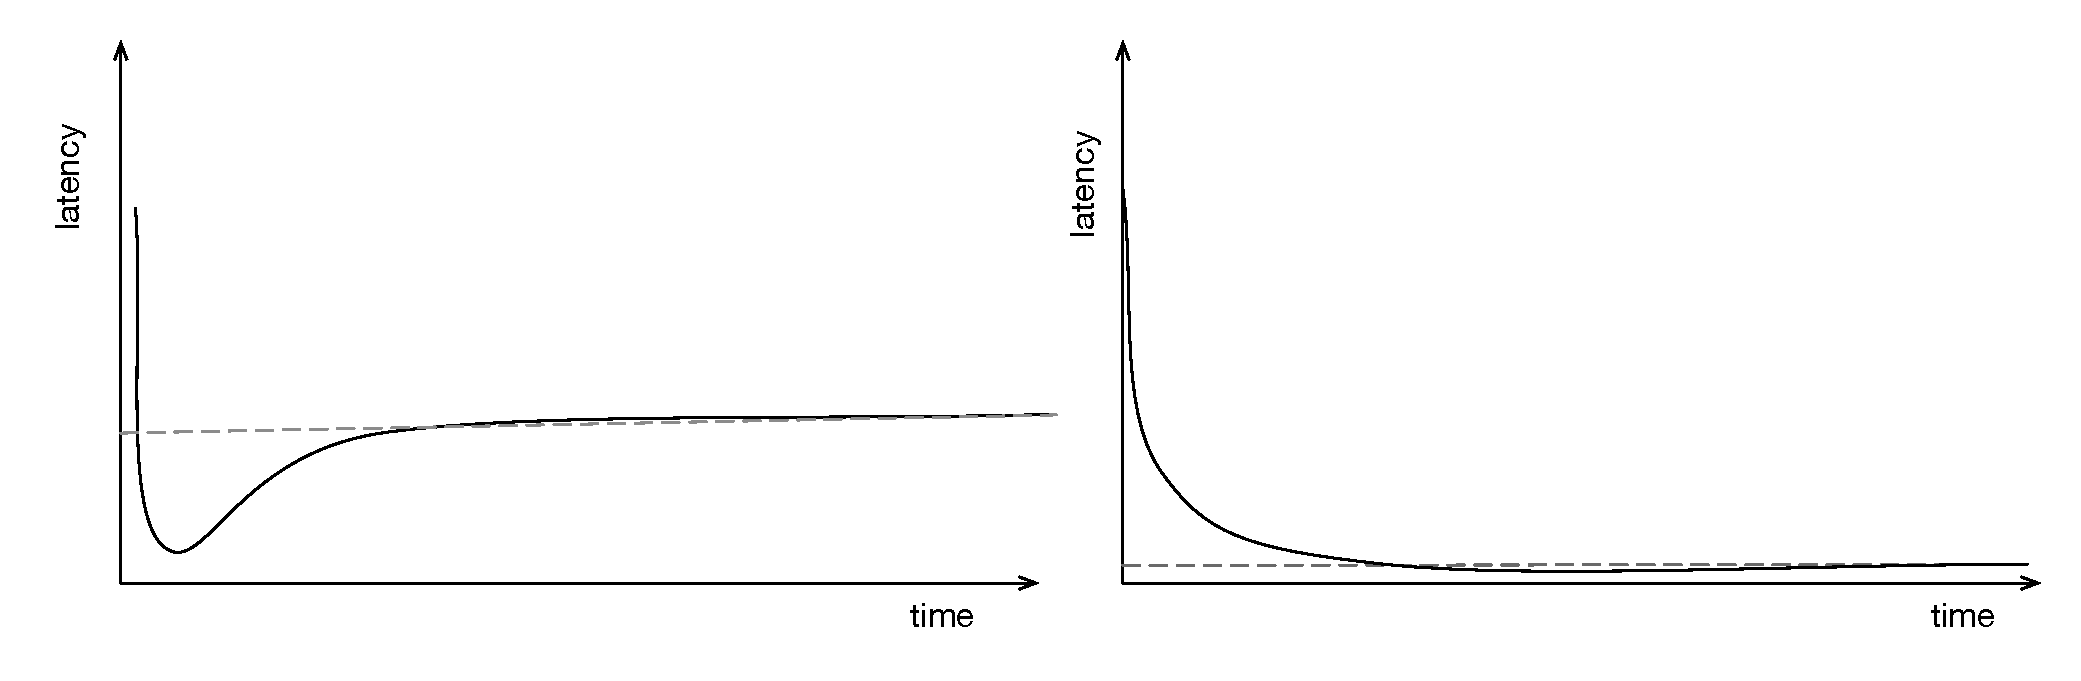
\includegraphics[width=\linewidth]{images/level2-pattern}
	\caption{Recognised Latency Pattern for SOAK Experiments} 
  	\label{fig:level2-pattern}
\end{figure}

\begin{figure}[hbt]
  \centering
	%\includegraphics[width=\linewidth]{images/level2-latency}
	\caption{...} 
  	\label{fig:level2-latency}
\end{figure}

\begin{figure}[hbt]
  \centering
	%\includegraphics[width=\linewidth]{images/level2-memory}
	\caption{...} 
  	\label{fig:level2-memory}
\end{figure}
\begin{figure}[hbt]
  \centering
	%\includegraphics[width=\linewidth]{images/level2-memory-density}
	\caption{...} 
  	\label{fig:level2-memory-density}
\end{figure}

\subsection{Level 3 - Single Visual Comparison}
	
The lowest level of analysis provided by \name focuses on the single graphical analysis. Section \ref{sec:analyser} shows two possible comparisons: Multi-variable and Multi-experiment. For soak test we only exploits the firs one, because we have already seen many example of inter-experiment analysis. Figure \ref{fig:level3-memory-latency-1} shows, the relation between memory and latency, by multi-plotting both the variable on the same chart.

It is clear in the Figure, that the two variables have very different behaviours: latency quickly reach the steady state condition, after a warm-up phase which is very high w.r.t the average of the entire execution. On the other hand, memory does not reach the Steady State so quickly. Java optimization policy seems to focus more on the speed of the execution than on memory optimization. Memory consumption is optimized slowly and only when it has reach the its maximum usage. This is more clear if we compare small experiment to the biggest ones. Figure \ref{fig:level3-memory-latency-2} shows how memory does not reaches the Steady State condition at all, however the optimisation is still in processing and divided in different phases while the JVM tries to understand the optimum.


\begin{figure}[hbt]
  \centering
	%\includegraphics[width=\linewidth]{images/level3-memory-latency}
	\caption{...} 
  	\label{fig:level3-memory-latency-1}
\end{figure}

\begin{figure}[hbt]
  \centering
	%\includegraphics[width=\linewidth]{images/level3-memory-latency}
	\caption{...} 
  	\label{fig:level3-memory-latency-2}
\end{figure}


\section{StepResponse Test Evaluation Results}\label{sec:stressres}
 Finally we show \name abilities presenting the results of Step Response tests in the Subsection \ref{sec:stressres}.


